\documentclass{beamer}

\usepackage[utf8]{inputenc}
\usepackage{listings}
\usepackage{algorithm,algorithmic}
\usepackage{beamerthemesplit}

\setbeamertemplate{footline}[frame number]
\setbeamertemplate{headline}{}


%Information to be included in the title page:
\title{Reinforcement Learning using the example of Mancala}
\author{Viktor Kosin und Johanna Beier}
\date{04.09.2020}



\begin{document}

\frame{\titlepage}

\begin{frame}
\frametitle{Structure}
\begin{itemize}
\item Mancala rules
\item Q-learning
\item Backpropagation
\item Network
\item Training
\item Troubleshooting
\item Results / Improvement
\end{itemize}
\end{frame}

\begin{frame}
\frametitle{Mancala}
\begin{itemize}
\item ancient two player game
\end{itemize}
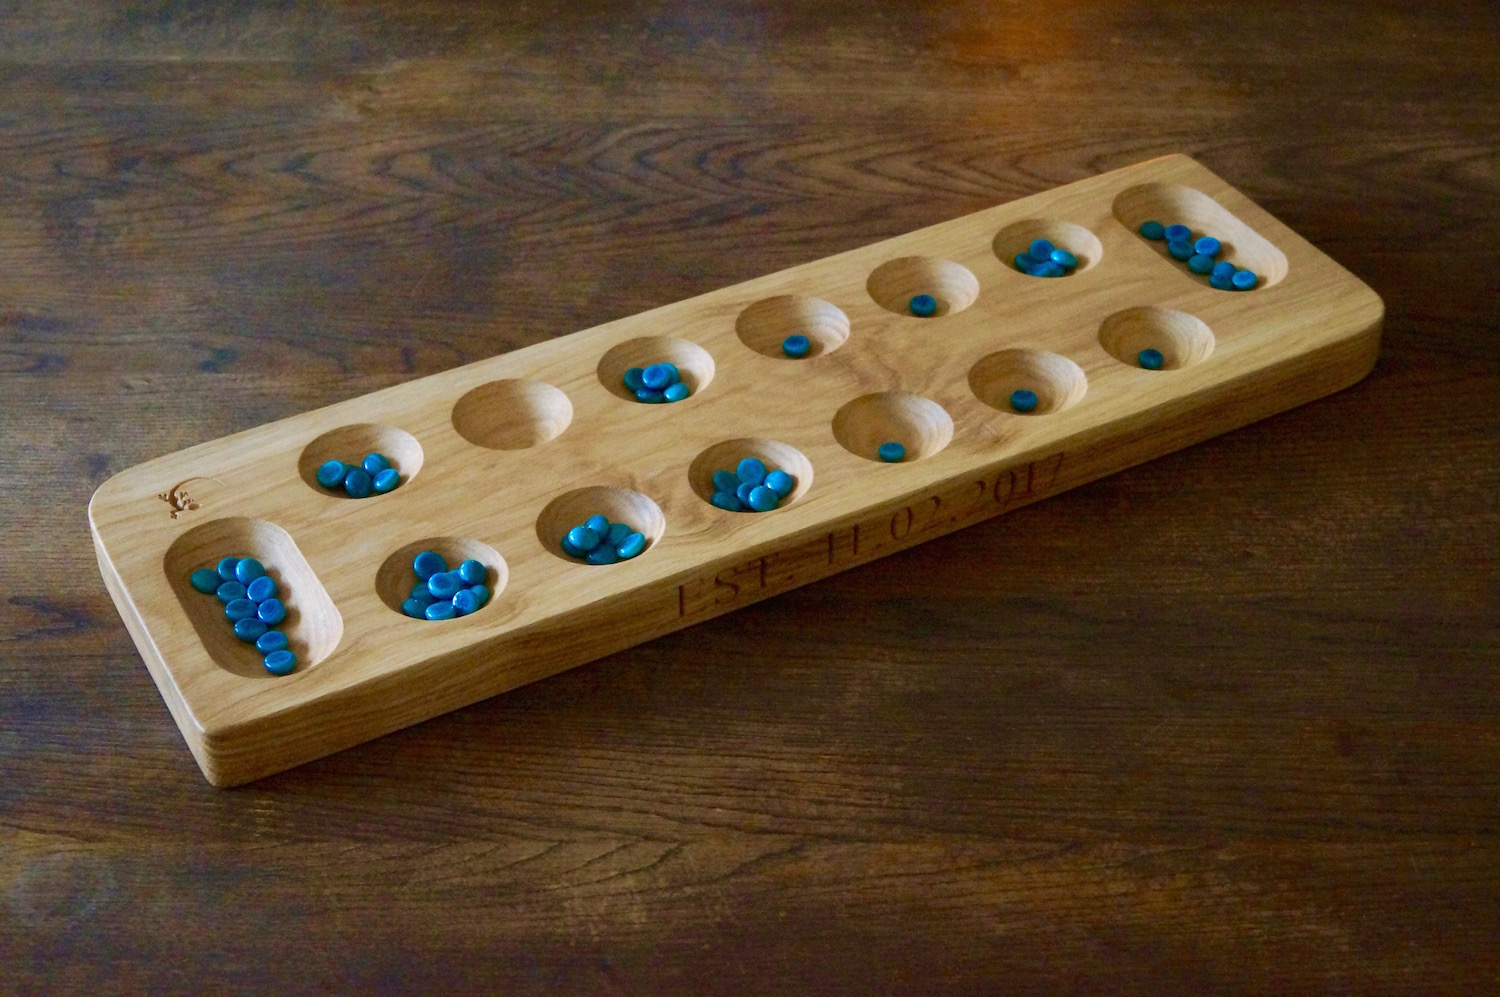
\includegraphics[scale=0.15]{board}
\begin{itemize}
\item \textbf{as vector:} $[6,6,6,6,6,6, | 6,6,6,6,6,6, |0,0]$
\item\textbf{Goal:} catch more then half of the beans (37) 
\end{itemize}
\end{frame}

\begin{frame}
\frametitle{Mancala Rules}
\begin{itemize}
\item choose non empty hole
\item collect all beans of a hole and drop one in each clockwise following hole
\item catch all beans of the last hole, if it contains $6$, $4$ or $2$ beans
\item going backwards: collect beans from all following holes with $6$, $4$ or $2$ beans, if there are no other holes in between
\item game ends if either one player has no more beans or one player catches at least $37$ beans
\item total sum of beans: catched beans $+$ beans on own side
\end{itemize}
\end{frame}

\begin{frame}
 \frametitle{MDP}
 \begin{itemize}
 \item Mancala can be represented as a Marcov Decision Process (MDP) 
 \item set of states S, set of actions per state A, action a $\in$ A
\item finite but very large number of states
 \item How does the Mancala agent learns to choose the best action?
 \end{itemize}
 \end{frame}

 \begin{frame}
 \frametitle{Reinforcement Learning}
 \begin{itemize}
 \item \textbf{Idea:} reward or punish some action
 \item \textbf{Goal of agent:} maximize total reward
 \item \textbf{possible rewards for Mancala:} Small reward for catching beans, bigger reward for winning the game, punish illegal actions and loosing
 \item use Q-Learning
 \end{itemize}
 \end{frame}
 
  \begin{frame}
  \frametitle{Q-learning}
 \begin{itemize}
 \item small state space: Q-table
  \item replace Q-table by Q-function 
  \begin{align}
  Q(s,a) \leftarrow Q(s,a)+\alpha [r+\gamma \max_{a'} Q(s',a') -Q(s,a)]
  \end{align}
 \item agents often need to learn actions that do not lead immediately to a reward
 \item allow a small amount of random actions (exploration rate)
 \end{itemize}
 \end{frame}
 
  \begin{frame}
 \frametitle{Netz}
\begin{itemize}
\item \textbf{activation function:} Sigmoidfunction
\item \textbf{loss function:} Meanvalue
\item size input layer: 14
\item size output layer: 6
\end{itemize}
 \end{frame}

  \begin{frame}
 \frametitle{play}
 \begin{itemize}
\item choose action by feeding the current board to the net and take the argmax of the output
\item get board and reward after action 
\item append board and reward to trainingslists
\item change player (turn board)
\end{itemize}
\end{frame}
 
 \begin{frame}
 \frametitle{Rewards and Discount}
 \begin{itemize}
 	\item choosing the right rewards is key for the Q-function to work properly
 	\begin{itemize}
 		\item too high rewards lead to large q-value estimations (maybe higher than the activation function would allow)\\
 		$\Rightarrow$ the network is going to increase q-values with every iteration
 		\item too low rewards lead to q-values close to zero
 		\item get 0.05 as reward for every caught bean and 10.0 for a winning action
 	\end{itemize}
 \item selecting the right discount and learning rate is difficult and depends on the reward strategy
 \end{itemize}
\end{frame}
 
 \begin{frame}
 \frametitle{Training}
 \begin{itemize}
\item let the agent play against itself and save pairs of actions and rewards
\item update for each board state and action the underlying Q-function
\item save each board state and dedicated Q-values as training data
\item feedforward a boardstate to the net
\end{itemize}
 \end{frame}
 
  \begin{frame}
 \frametitle{Backpropagtion}
 \begin{itemize}
 \item[\textbf{1. Step}] Generate training data: for a given input set an expected output (e.g. with Q-function)
 \item[\textbf{2. Step}] Calculate for the input $a^{x,1}$:
 \begin{itemize}
 \item activation $a^{x,l}$ of layer $l=2,3,...,L$ by
 $$a^{x,l} = \sigma(z^{x,l}),\quad z^{x,l} = w^l a^{x,l-1} + b^l$$
 \item Output error $\delta^{x,L} = \nabla_a C_x \odot \sigma'(z^{x,L})$
 \item Backpropagate error to each layer: 
 $$\delta^{x,l} = ((w^{l+1})^T \delta^{x,l+1}) \odot \sigma' (z^{x,L})$$
 \end{itemize}
 \item[\textbf{3. Step}] Use error of each layer to update weights and biases 
 \end{itemize}
 \end{frame} 
 
 \begin{frame}
\frametitle{Results for a straightforward adaptation}
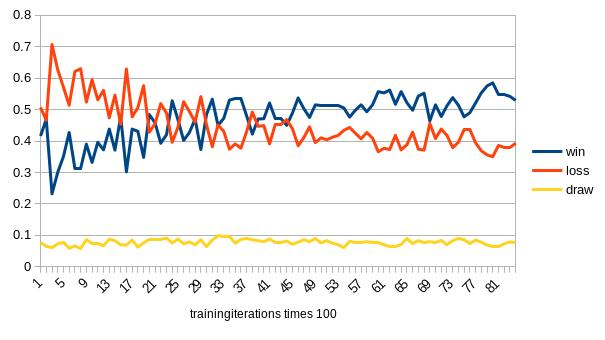
\includegraphics[scale=0.65]{gewinnrate.jpg}
\begin{itemize}
\item simple q-learning tends to stagnate very early, gets worse after some time
%\item the q-values of multiple possible actions get close to 1
\item a 'large' learning rate doesn't always improve the rate
\end{itemize}
\end{frame}
 
\begin{frame}
\frametitle{Origins of problems}
\begin{itemize}
\item couldn't identify any coherence
\item to see how the network learns Mancala, we need to simplify the game
\end{itemize}
\end{frame} 
 
 \begin{frame}
 \frametitle{simple game}
\begin{itemize}
\item $[1,1,5,1,1,1|1,1,5,1,1,1|0,0]$
\item play against random
\item network ist startplayer
\item obvious way of playing at least tied
\item after some trainingiterations the second player does not win at all
\item $\rightarrow$ network is ok
\end{itemize}
 \end{frame}

 \begin{frame}
 \frametitle{simple board}
 \begin{itemize}
\item reduce the board size: $[2,2|2,2|0,0]$
\item obvious way of loosing the game: choose first hole
\item compare guessed Q-Values with choice of hole
\item Q-function decides for wrong side $\rightarrow$ solve this error
\item net performs good, if it starts in the right direction
\item use flexible exploration rate
\end{itemize}
 \end{frame}

 \begin{frame}
 \frametitle{simple board results}
 \center{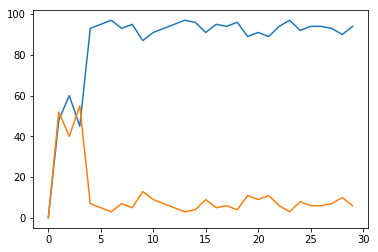
\includegraphics[scale=0.5]{kleinesNetz10}}
\begin{itemize}
\item $1$ hidden layer with 10 neurons
\item $1$ Unit = 100 Trainingiterations
\end{itemize}
 \end{frame}

 \begin{frame}
 \frametitle{simple board results: jump}
 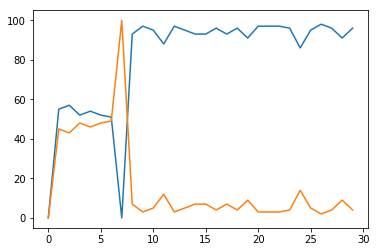
\includegraphics[scale=0.7]{kleinesNetz202}
 \end{frame}

 \begin{frame}
 \frametitle{Mancala with $4$ beans per hole}
 \begin{itemize}
\item  $[4,4,4,4,4,4|4,4,4,4,4,4|0,0]$
\item transfer findings to this game (flexible exploration rate, ...)
\item learns something but oscillates 
\item  learns better if starts in the right direction
\end{itemize}
 \end{frame}

 \begin{frame}
 \frametitle{Mancala with $4$ beans per hole}
 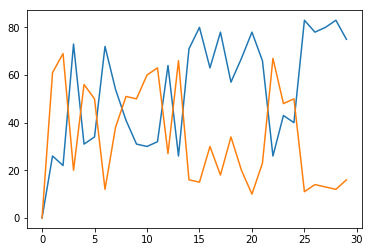
\includegraphics[scale=0.7]{4holeos}
 \end{frame}

\begin{frame}
\frametitle{improved Mancala with $4$ beans per hole}
\begin{itemize}
\item Idea: reduce learining rate if net performs good otherwise increase learning rate
\item reward only winning not catching beans
\end{itemize}
\end{frame}

\begin{frame}
\frametitle{flexible parameters}
\lstinputlisting[language = python]{python1.py}
\end{frame}

 \begin{frame}
\frametitle{improved Mancala with $4$ beans per hole}
 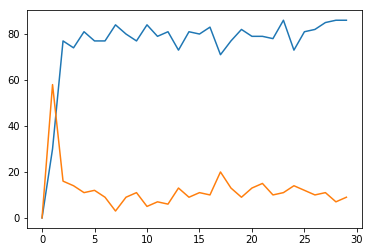
\includegraphics[scale=0.7]{4holestrainingconvergence}
\begin{itemize}
\item keep in mind: Mancala ist still more complex and will possible take more time to converge
\end{itemize}
 \end{frame}

\begin{frame} 
\frametitle{Adapting learning of Mancala}
\begin{itemize}
\item generating a random network of size $[14,10,6]$
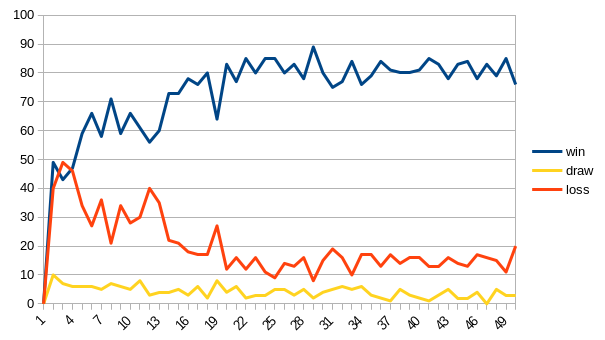
\includegraphics[scale=0.5]{mancala_konvergenz}
\end{itemize}
\end{frame}
\begin{frame}
\frametitle{Possible improvements}
\begin{itemize}
\item use multiple network to guess optimal parameters of q-function and network, e.g:
\begin{itemize}
\item exploration rate, rewards
\item discount, learning rate
\end{itemize}
\item use tree search algorithm to guess rewards over multiple future actions
\end{itemize}
\end{frame}
\begin{frame}
\frametitle{Approved agents of other Mancala like games}
\begin{itemize}
\item MinMax
\item Monte Carlo Tree Search
\item Asynchronous Advantage Actor-Critic
\begin{itemize}
\item runs parallel agents
\item 3 networks work in concert: input, action and critic
\end{itemize}
\end{itemize}
\end{frame}
\begin{frame}
\frametitle{Quellen}
\begin{itemize}
\item neuralnetworksanddeeplearning.com/chap2.html
\item towardsdatascience.com/the-ancient-game-and-the-ai-d7704bea280d
\item https://1tr7g949k6uv1s2cx31wn2yt-wpengine.netdna-ssl.com/wp-content/uploads/2017/02/handmad
\end{itemize}
\end{frame}
\end{document}